\section{Bernstein-Vaziraniアルゴリズム}
\label{sec:bernstein-vazirani}
Bernstein-Vaziraniアルゴリズムは，隠されたビット列を特定するための量子アルゴリズムである．古典コンピュータでは，隠されたビット列を特定するために複数回の問い合わせが必要であるのに対し，量子コンピュータによるBernstein-Vaziraniアルゴリズムの計算では1回の問い合わせで隠されたビット列を特定することができる．
図中の$U_{f_s}$は，隠れた正解のビット列$s=(s_1,s_2,s_3)\in\{0,1\}^3$に対して，入力ビット列$x=(x_1,x_2,x_3)\in\{0,1\}^3$から$f_s(x)=s_1x_1\oplus s_2x_2\oplus s_3x_3 \in \{0,1\}$を計算する量子オラクルである．
3ビットの場合の量子回路を図\ref{fig:bernstein-vazirani-circuit}に示す．
\begin{figure}[H]
\centering
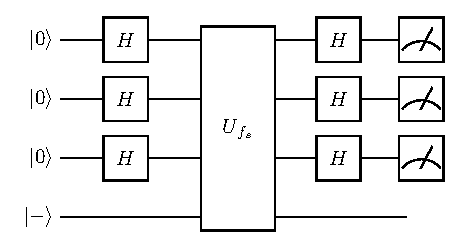
\includegraphics[width=0.8\textwidth]{figures/03-quantum-subroutines/bernstein-vazirani-circuit.pdf}
\caption{3ビットのBernstein-Vaziraniアルゴリズムの量子回路}
\label{fig:bernstein-vazirani-circuit}
\end{figure}

Bernstein-Vaziraniアルゴリズムの手順は以下の通りである．
\begin{enumerate}
\item $\ket{0}^{\otimes n}$に初期化された量子ビット（入力レジスタ）と，補助量子ビットを$\ket{-}$を準備する．
\item 入力レジスタにアダマール変換$H^{\otimes n}$を適用する．
\item 量子オラクル$U_{f_s}$を適用する．
\item 再び入力レジスタに$H^{\otimes n}$を適用する．
\item 入力レジスタを測定する．
\end{enumerate}

\begin{align*}
    \ket{\psi_1}\coloneq\ket{0}^{\otimes n}\ket{-} \xrightarrow{H^{\otimes n}} \bigg( \frac{1}{\sqrt{2^n}}\sum_{x\in\{0,1\}^n}\ket{x}\bigg)\ket{-} \quad (\eqcolon{\psi_2})
\end{align*}
手順2で重ね合わせ状態を作る．これにより，量子オラクル$U_{f_s}$は全ての入力に同時に作用することができる．（量子並列性）
\begin{align*}
    \ket{\psi_2} \xrightarrow{U_{f_s}}
    \ket{\psi_2} \bigg( \frac{1}{\sqrt{2}}\left(\ket{0 \oplus f_s(x)} - \ket{1 \oplus f_s(x)}\right) \bigg)\quad (\eqcolon{\psi_3}) \\[8pt]
\end{align*}
$f_s(x) \in \{0,1\}$なので，$f_s(x) = 0$と$f_s(x) = 1$の場合に分けて考えると
\begin{align*}
    \ket{\psi_3} 
    &=
    \begin{dcases*}
        \dfrac{1}{\sqrt{2^n}}\sum\limits_{x\in\{0,1\}^n}\ket{x}\dfrac{1}{\sqrt{2}}\left(\ket{0} - \ket{1}\right) & (\text{if $f_s(x) = 0$}) \\[8pt]
        \dfrac{1}{\sqrt{2^n}}\sum\limits_{x\in\{0,1\}^n}\ket{x}\dfrac{1}{\sqrt{2}}\left(\ket{1} - \ket{0}\right) & (\text{if $f_s(x) = 1$})
    \end{dcases*}\\[8pt]
    &= \begin{dcases*}
        \dfrac{1}{\sqrt{2^n}}\sum\limits_{x\in\{0,1\}^n}\ket{x}\ket{-} & (\text{if $f_s(x) = 0$}) \\[8pt]
        \dfrac{1}{\sqrt{2^n}}\sum\limits_{x\in\{0,1\}^n}\ket{x}(-\ket{-}) & (\text{if $f_s(x) = 1$})
    \end{dcases*}\\[8pt]
\end{align*}
これら二つの場合をまとめて$(-1)^{f_s(x)}$で表すと，量子オラクル適用後の状態は
\begin{align*}
    \ket{\psi_3} =\dfrac{1}{\sqrt{2^n}}\sum_{x\in\{0,1\}^n} (-1)^{f_s(x)}\ket{x}\ket{-}
\end{align*}
$n$量子ビットの場合，$f_s(x) = s_1x_1 \oplus s_2x_2 \oplus \cdots \oplus s_nx_n$なので
\begin{align*}
    \ket{\psi_3}
    &= \frac{1}{\sqrt{2^n}}\sum_{x\in\{0,1\}^n} (-1)^{\bigoplus_{i=1}^n s_i x_i}\ket{x}\ket{-} \\
    &= \frac{1}{\sqrt{2^n}}\sum_{x\in\{0,1\}^n} \bigg(\prod_{i=1}^n (-1)^{s_i x_i}\bigg) \ket{x}\ket{-} \\
\end{align*}
$\ket{x} = \bigotimes_{i=1}^n \ket{x_i}$と表記すると，$\prod_{i=1}^n (-1)^{s_i x_i}$も$\bigotimes_{i=1}^n (-1)^{s_i x_i}$と書けるので，量子状態$\ket{\psi_3}$は
\begin{align*}
    \ket{\psi_3} 
    = \frac{1}{\sqrt{2^n}}\sum_{x\in\{0,1\}^n} \bigg( \bigotimes_{i=1}^n (-1)^{s_i x_i} \ket{x_i} \bigg) \ket{-} 
\end{align*}
$x^T=(x_1,\ldots,x_n) \in \{0,1\}^n$の各成分はそれぞれ$0$または$1$をとるため，ビット列全体にわたる総和は各量子ビットについての和に分けられる．また，$1/\sqrt{2^n}=(1/\sqrt{2})^n$なので
\begin{align*}
    \ket{\psi_3} 
    &= \bigotimes_{i=1}^n \bigg( \frac{1}{\sqrt{2}} \sum_{x_i = 0}^{1} (-1)^{s_i x_i} \ket{x_i} \bigg) \ket{-} \\
    &= \bigotimes_{i=1}^n \dfrac{\ket{0} + (-1)^{s_i} \ket{1}}{\sqrt{2}} \ket{-}
\end{align*}
$\dfrac{\ket{0} + \ket{1}}{\sqrt{2}} = H\ket{0}, \quad \dfrac{\ket{0} - \ket{1}}{\sqrt{2}} = H\ket{1}$より，$\dfrac{\ket{0} + (-1)^{s_i} \ket{1}}{\sqrt{2}} = H\ket{s_i}$となるので
\begin{align*}
    \ket{\psi_3}
    &=\bigotimes_{i=1}^n \dfrac{\ket{0} + (-1)^{s_i} \ket{1}}{\sqrt{2}} \ket{-} 
    &= \bigotimes_{i=1}^n H\ket{s_i} \ket{-} \\
    &= H^{\otimes n} \ket{s} \ket{-}
\end{align*}
と書けるので，再度入力レジスタにアダマール変換$H^{\otimes n}$を適用すると，$HH = I$より
\begin{align*}
    \ket{\psi_3}\xrightarrow{H^{\otimes n}} 
    &\left(H^{\otimes n}\right) \left(H^{\otimes n}\right) \ket{s} \ket{-} \\
    &= \left(HH\right)^{\otimes n} \ket{s} \ket{-} \\
    &= \ket{s} \ket{-}
\end{align*}
よって，入力レジスタの測定を計算基底で行えば，秘密のビット列$s$が得られる．
古典コンピュータでは，$s$を得るためには，最悪の場合$n$回のオラクル呼び出しが必要であるのに対し，量子コンピュータでは量子並列性により，一度のオラクル呼び出しで$s$を求めることができる．
\newpage